\documentclass{beamer}
\usepackage[utf8]{inputenc}
\usetheme{default}
\usecolortheme{dove}
\usepackage{textpos}
\usepackage{grid-system}
\usepackage[official]{eurosym}


% po4a: environment frame
% po4a: environment Row
% po4a: environment Cell


\title{Freifunk Darmstadt}
\author{
\includegraphics[width=4cm]{images/logo}}
%\institute[Inst.]{Freifunk Darmstadt}
\date{29. Januar 2014}

\begin{document}

\begin{frame}
\maketitle
\end{frame}

\addtobeamertemplate{frametitle}{}{%
\begin{textblock*}{100mm}(0.93\textwidth,-0.5cm)

\includegraphics[height=1cm]{images/logo}
\end{textblock*}}

\begin{frame}{Themen}
\tableofcontents
\end{frame}

\section{Was ist Freifunk?}
\begin{frame}{Was ist Freifunk?}
\begin{itemize}
	\item Teil einer weltweiten Bewegung zur Etablierung von offenen und freiem Netzzugang
	\item Neben der Bereitstellung eines Internetzugangs auch Plattform für lokale Dienste
	\item dezentral und gemeinschaftlich von Bürgern, Vereinen, Unternehmern und Institutionen betrieben
	\item robuste Netzwerktopologie durch Verwendung von Mesh-Netzwerken und dezentralen Routingalgorithmen
	\item Freifunk Darmstadt: Initiative des Chaos Darmstadt e.V.
\end{itemize}
\end{frame}


\begin{frame}{Freifunk in Deutschland}
\vfill
\begin{center}
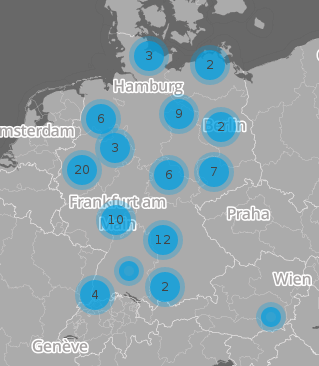
\includegraphics[height=0.6\textheight]{images/map}$\;$
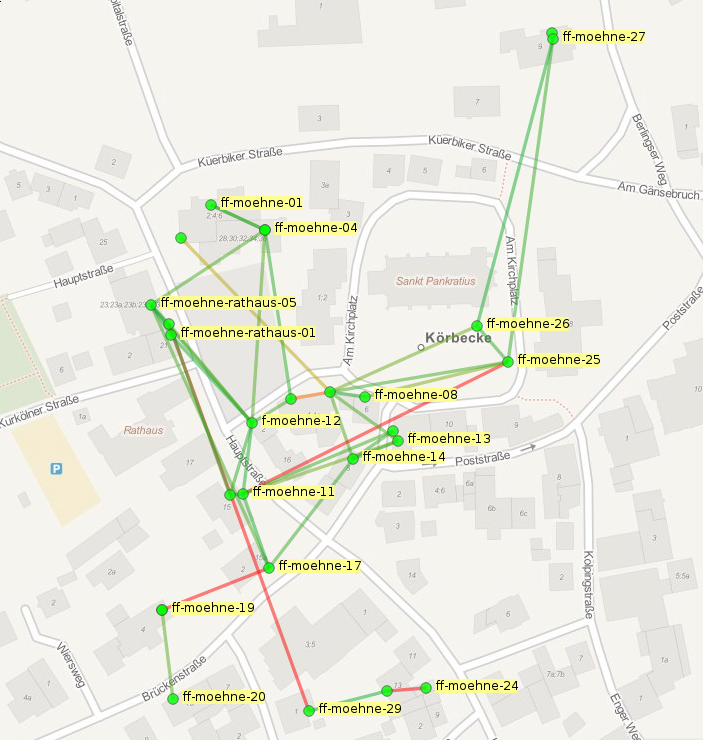
\includegraphics[height=0.6\textheight]{images/moehne}
\end{center}
\vfill
\end{frame}

\section{Projektbeschreibung}
\begin{frame}{Projektbeschreibung}
\vfill
\begin{center}
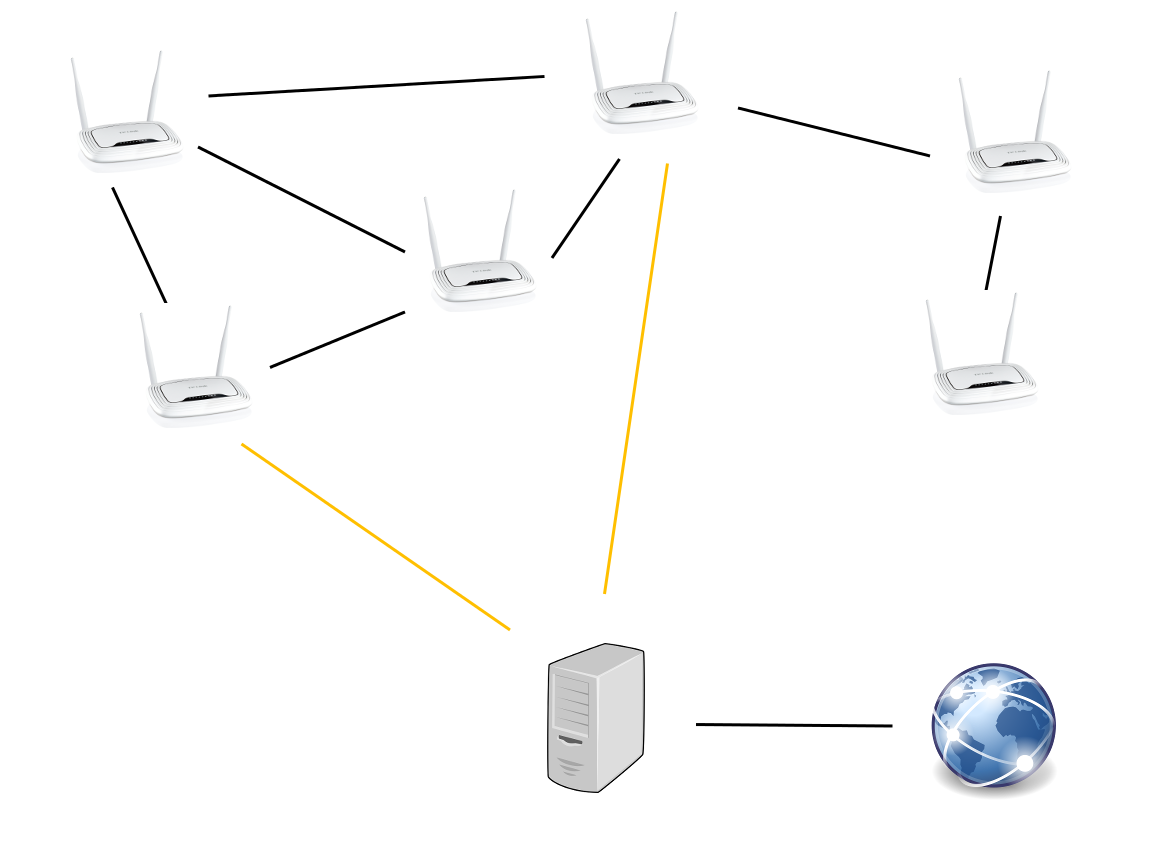
\includegraphics[height=0.7\textheight]{images/meshing}
\end{center}
\vfill
\end{frame}

\section{Aktueller Stand}
\begin{frame}{Aktueller Stand}
\vfill
\begin{center}
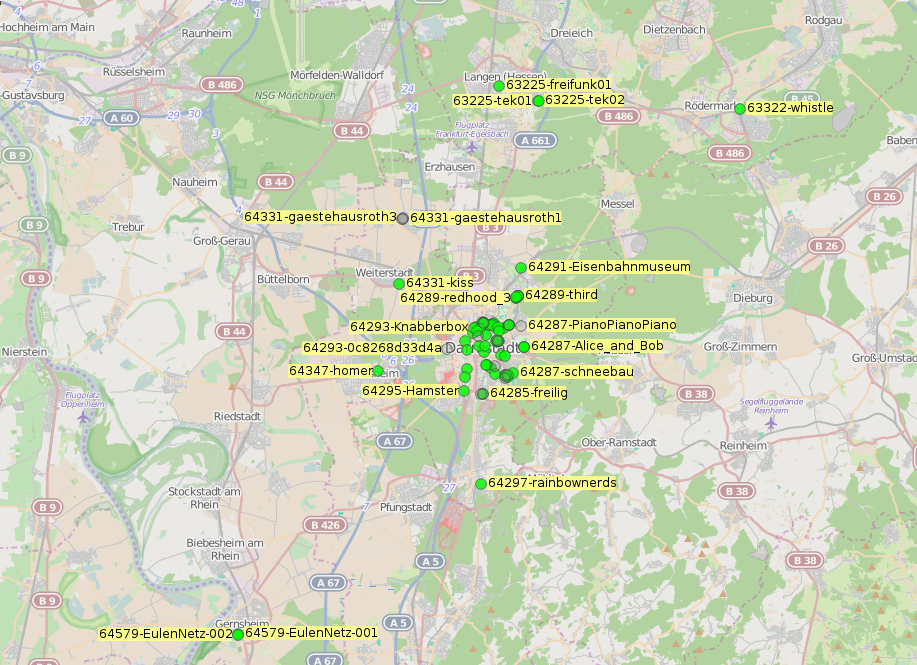
\includegraphics[height=0.75\textheight]{images/2015-01-26-map}$\;$
\vfill
ca. 80 Accesspoints
\end{center}
\end{frame}

\begin{frame}{Aktueller Stand - Darmstadt}
\vfill
\begin{center}
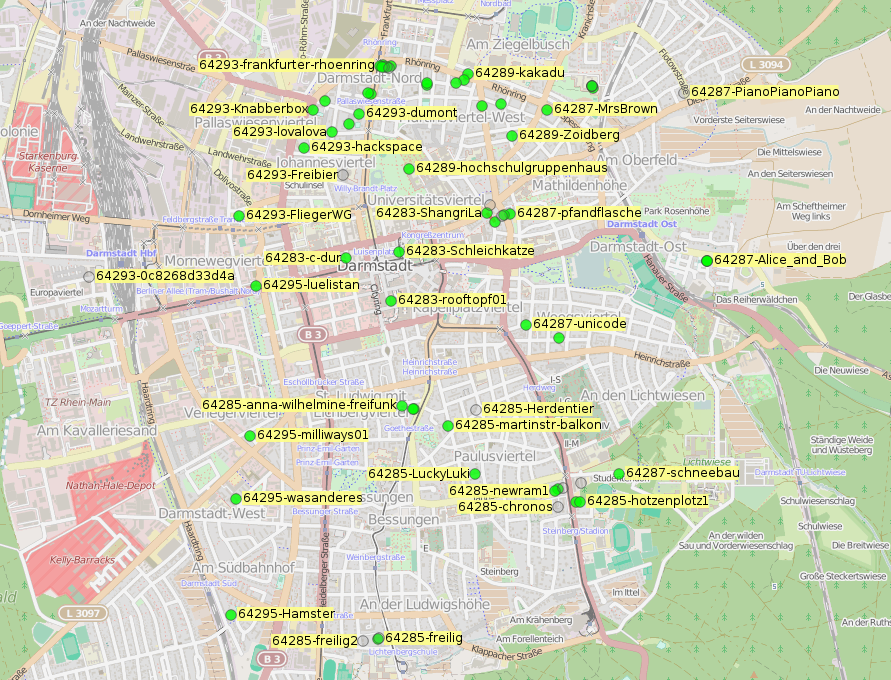
\includegraphics[height=0.75\textheight]{images/2015-01-26-darmstadt}$\;$
\vfill
\end{center}
\end{frame}

\begin{frame}{Aktueller Stand - K6}
\vfill
\begin{center}
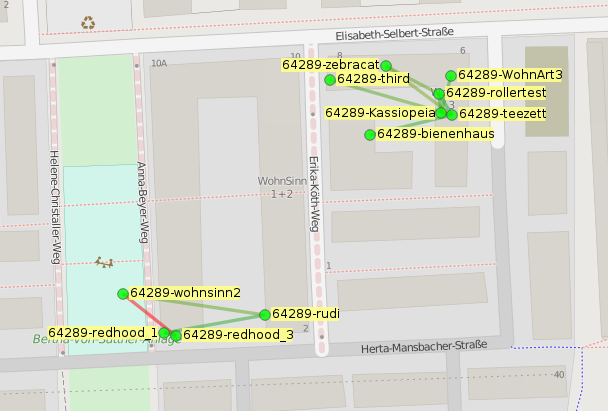
\includegraphics[height=0.75\textheight]{images/2015-01-26-wohnart3}$\;$
\vfill
\end{center}
\end{frame}

\section{Ausbauplan}
\begin{frame}{Ausbauplan}
\vfill
\begin{itemize}
	\item öffentliche Plätze, Staatstheater, Haltestellen, Krankenhäuser
	\item Hotels, Gaststätten, öffentliche Einrichtungen
	\item Parks (z.B. Herrengarten, Prinz-Emil-Garten)
	\item private Wohnungen, Studentenwohnheime
	\item hochgelegene Plätze für Richtfunk (z.B. Langer Ludwig, Kirchtürme, Hochzeitsturm, h$\_$da Hochhaus)
\end{itemize}
\vfill
\pause
\begin{itemize}
	\item Anlieger stellen der Freifunk-Community Standorte zur Verfügung und betreiben eigene Freifunk-Router
	\item Durchführung von Informationsveranstaltungen und Workshops über Freifunk und den sicheren Umgang damit
\end{itemize}
\vfill
\end{frame}

\section{Verwendete Router-Hardware}
\begin{frame}{Verwendete Router-Hardware}
Handelsübliche Modelle im 2.4GHz- und 5GHz-Band
\vfill
Für den Heimbedarf oder kleinere öffentliche Bereiche:
\begin{itemize}
\item bis zu 15-25 Clients pro Gerät
\item 30-70\euro{}
\end{itemize}
\vfill

Größere Inneninstallationen:
\begin{itemize}
\item bis zu 100 Clients pro Gerät und Frequenzband
\item ca. 250\euro{}
\end{itemize}
\vfill

Außeneinsatz:
\begin{itemize}
\item bis zu 100 Clients pro Gerät und Frequenzband
\item Kosten abhängig von Frequenzband, Geschwindigkeit und Antennentyp, 100-600\euro{}
\end{itemize}
\vfill
\end{frame}

\begin{frame}{Beispiel: Luisenplatz}
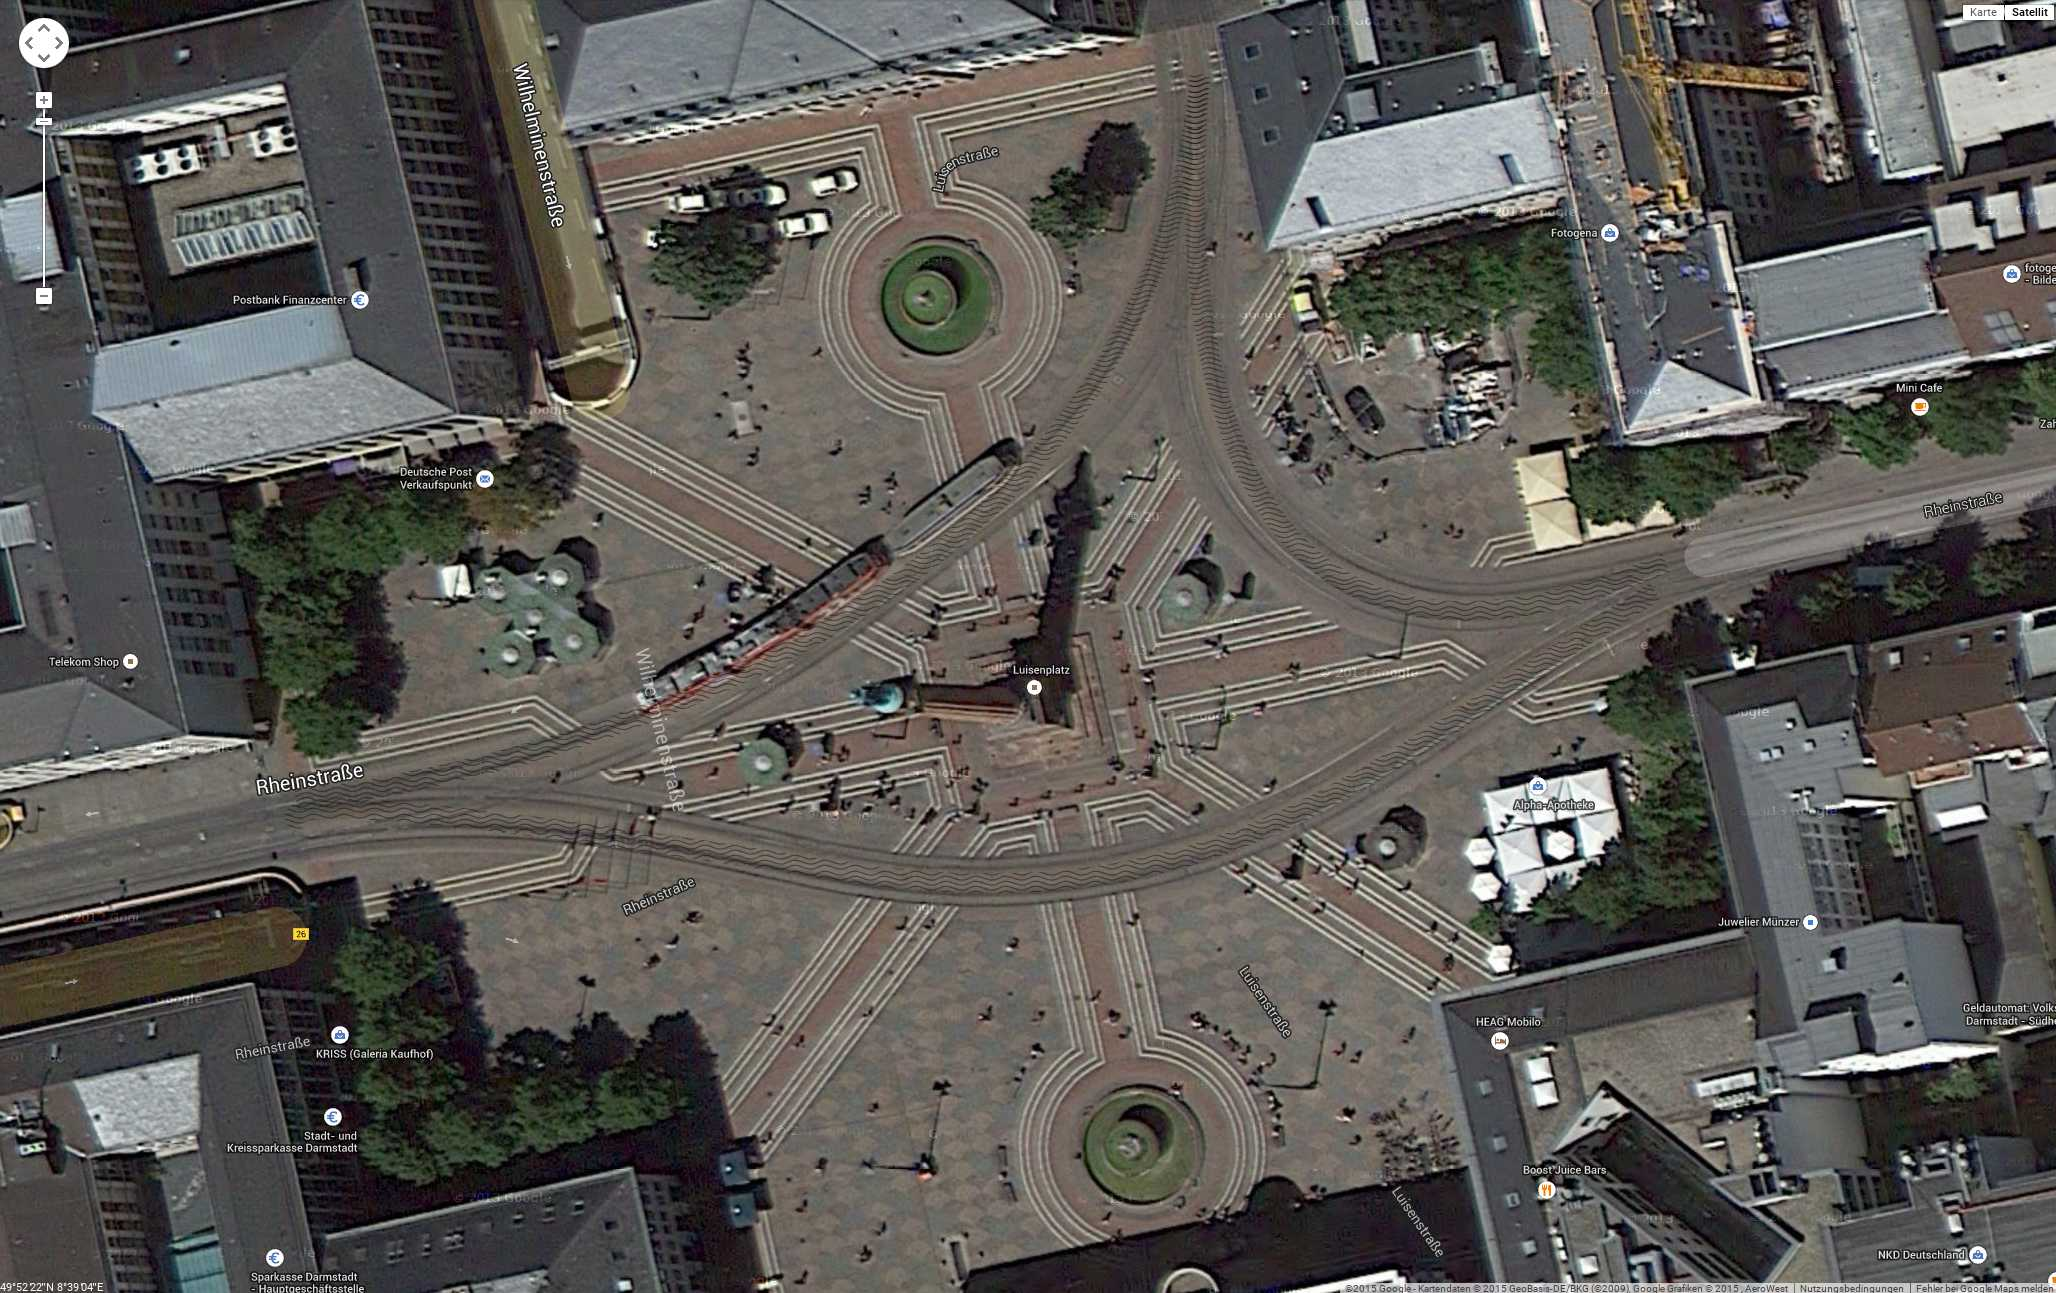
\includegraphics[height=0.75\textheight]{images/map_luisenplatz_1.jpg}$\;$
\end{frame}

\begin{frame}{Beispiel: Luisenplatz}
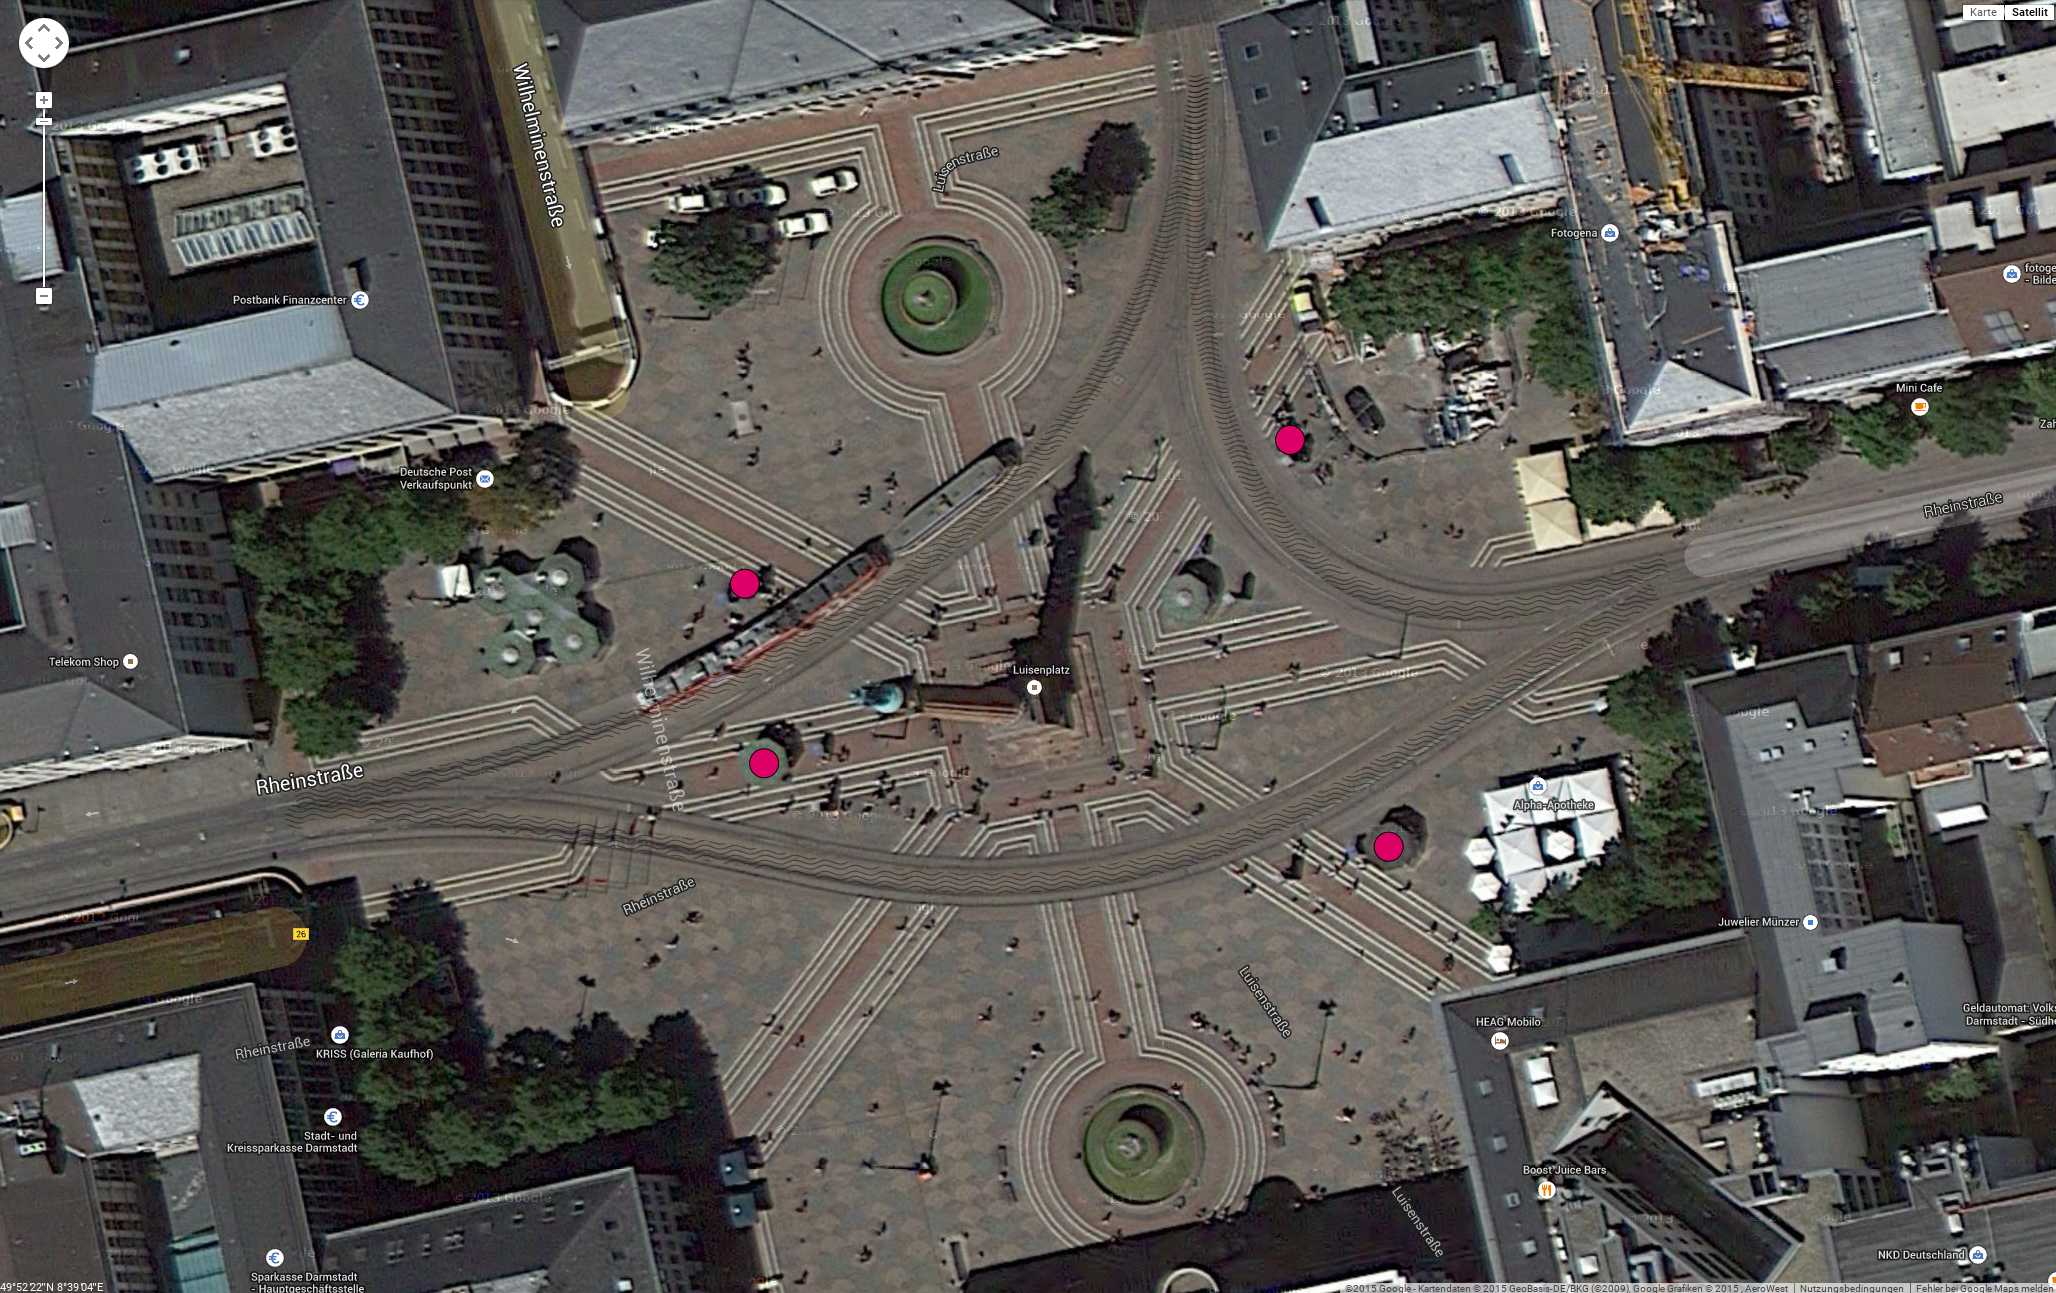
\includegraphics[height=0.75\textheight]{images/map_luisenplatz_2.jpg}$\;$
\end{frame}

\begin{frame}{Beispiel: Luisenplatz}
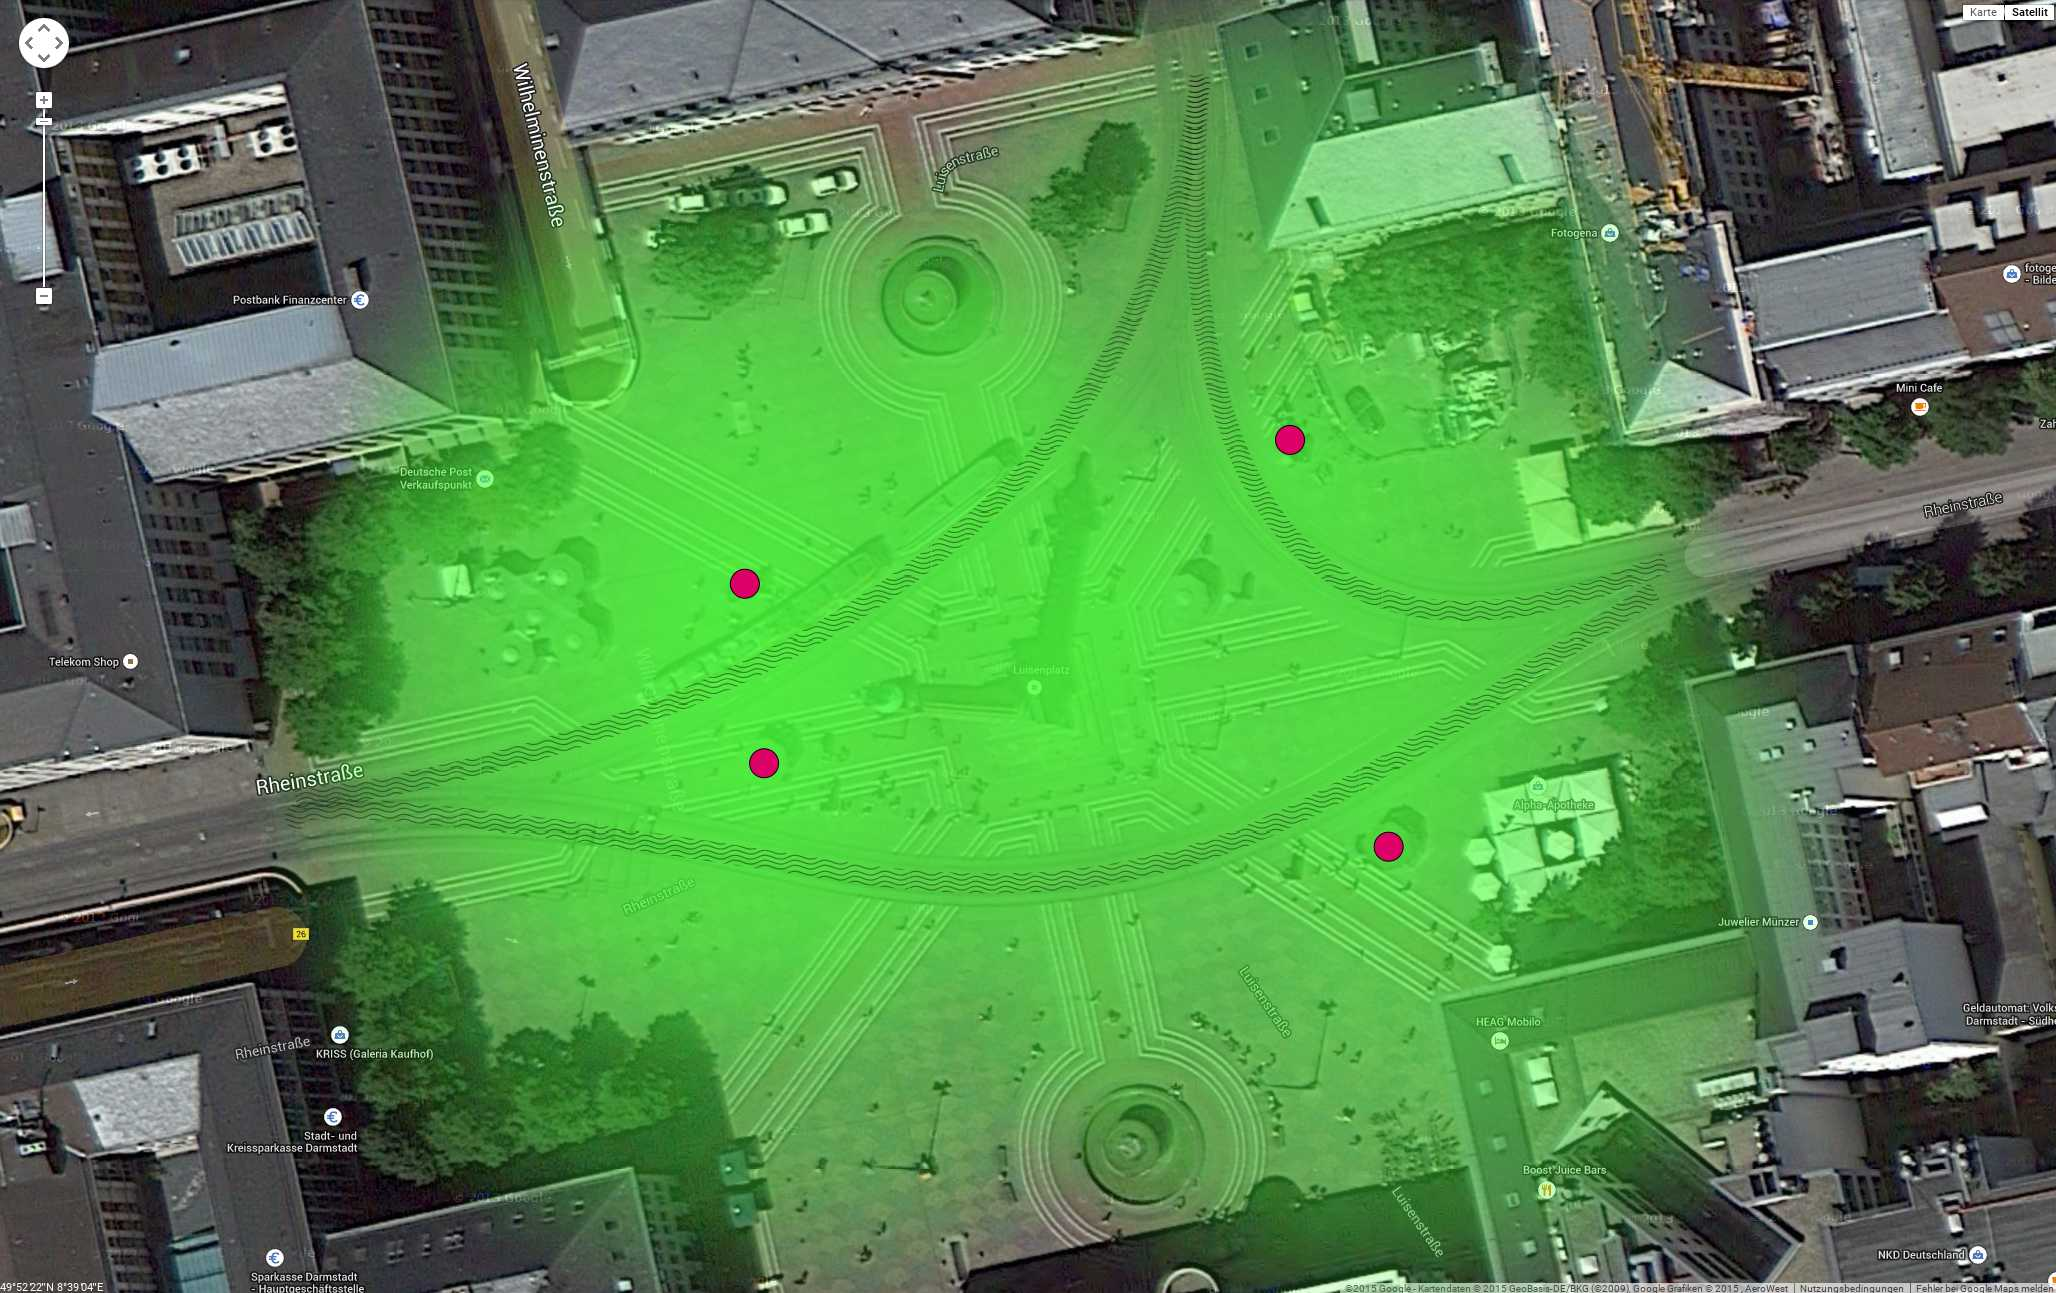
\includegraphics[height=0.75\textheight]{images/map_luisenplatz_3.jpg}$\;$
\end{frame}

\section{Anforderungen an die Stadt}
\begin{frame}{Anforderungen an die Stadt}
\vfill
\begin{center}
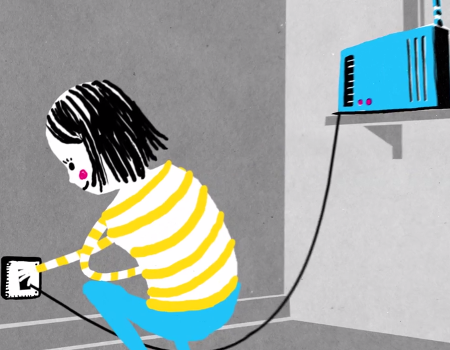
\includegraphics[height=0.4\textheight]{images/setup}$\;$
\vfill
\end{center}
\begin{itemize}
\item Bereitstellung von Standorten/Montageflächen
\item Bereitstellung von Strom und Internetanbindung/Richtfunk
\item Erwerb oder Sponsoring der notwendigen Hardware
\item standortabhängig Durchführung fachgerechter Montagearbeiten
\end{itemize}
\vfill
\end{frame}

\section{Organisation}
\begin{frame}{Organisation}
\vfill
\begin{itemize}
\item das Freifunk-Kernteam ist zuständig für
	\begin{itemize}
	\item Netzwerkinfrastruktur
	\item Firmwareaktualisierung
	\item Communitymanagement
	\item Support
	\end{itemize}
\vfill
\item die Freifunk-Community besitzt die Knoten und ist für deren Betrieb verantwortlich
\end{itemize}
\vfill
\end{frame}

\begin{frame}{Organisation - Infrastruktur}
\vfill
\begin{itemize}
	\item Multiple VPN-Endpunkte
	\item Redundante Internetanbindung
	\item kontinuierliches Monitoring aller kritischen Systeme
\end{itemize}
\begin{center}
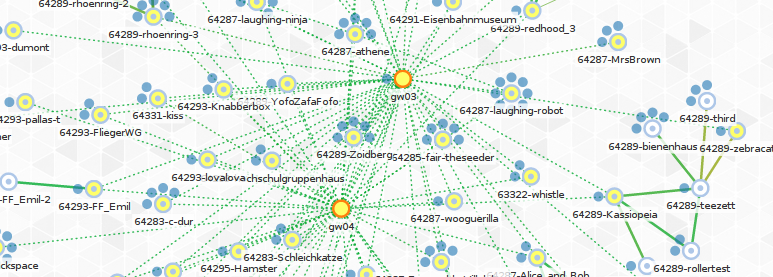
\includegraphics[width=\textwidth]{images/2015-01-28-graph}
\end{center}
\vfill
Zeit bis zum Failover bei Ausfall einer Internetanbindung: max. 60s
\vfill
\end{frame}

\begin{frame}{Organisation - Firmware}
\vfill
\begin{itemize}
	\item Gluon Framework, basierend auf OpenWrt
	\item Entwicklung durch deutschlandweite Community
	\item integrierter Updatemechanismus
	\begin{itemize}
		\item Integrität und Authentizität durch kryptographische Signatur sichergestellt
	\end{itemize}
\end{itemize}
\vfill
Ausrollen neuer Firmware-Releases binnen 24 Stunden (bei SSH-Zugang auf die Knoten on-demand) 
\vfill
\end{frame}
	
\begin{frame}{Organisation - Communitymanagement}
\vfill
\begin{itemize}
\item Regelmäßige Informationsveranstaltungen
\item Support bei unseren Treffen und Online
\item Öffentlichkeitsarbeit
\end{itemize}
\vfill
\end{frame}

\end{document}
